%-*- latex -*-
\chapter{DOSBox and MASM}
\section {Getting Your Computer Ready}
We will be using the Microsoft Assembler (MASM) which can be downloaded from Canvas.  Unzip it where you'd like to work on your projects and make a note of the absolute address of the file (\verb|C:\Users\etc|)
\index{installing DOSBox|(}
\subsection{Macs}
If you have OSX, I recommend downloading the .dmg file from the \href{https://www.dosbox.com/download.php?main=1}{official DOSBox Downloads page}.  You can install it as you would install a normal .dmg.  \\
\indent After installation hit 'command' + 'shift' + '.' to show hidden files.  Navigate to the hidden {\code Library} folder in your {\code Users/username/} folder.  In there open Preferences and scroll down to a file called 'DOSBox x.xx-x-x Preferences' and open it as text file (the x's are the version of DOSBox you downloaded).\\
Scroll to the bottom and add:
\begin{verbatim}
mount c /Users/yourname/MASM611
set PATH=%PATH%;C:\BIN
c:
\end{verbatim}
Don't forget to replace \verb|/Users/yourname/MASM611| with where you unzipped the MASM folder you downloaded.  

\subsection{PCs}
If you have a PC, I recommend downloading the .exe file from the \href{https://www.dosbox.com/download.php?main=1}{official DOSBox Downloads page}.  You can install it as you would install a normal .exe.  \\
After installation you can go to the Start Menu and select the DosBox folder and then DOSBox Options.  This will open a text file, scroll to the bottom and add: 
\begin{verbatim}
mount c C:\Users\yourname\MASM611
set PATH=%PATH%;C:\BIN
c:
\end{verbatim}
Don't forget to replace \verb|C:\Users\yourname\MASM611| with where you unzipped the MASM folder you downloaded.  \\
If you don't have administrative priviledges on your computer there is a \href{https://portableapps.com/apps/games/dosbox_portable}{Portable Apps version}. 
\index{installing DOSBox|)}
\subsection{Testing DOSBox}
Open DOSBox and test it out by typing {\code ml} at the prompt and then {\code <enter>}, it should say something like:
\begin{verbatim}
Microsoft (R) Macro Assembler Version 6.11
Copyright (C) Microsoft Corp 1981-1993. All rights reserved.

usage: ML [ options ] filelist [ /link linkoptions]
Run "ML /help" or "ML /?" for more info
\end{verbatim}
Congratulations you have successfully installed DOSBox and MASM!  One final note, since it is DOS, the preferred number of characters of a filename is 8.  While it is possible to have longer names, it will make your life easier if all of your assembly program filenames are less than or equal to eight characters (eg {\code filename.asm} is fine). 

\section{Using MASM}
\subsection{Assembling}
First download "hello.asm" from Canvas and put it in your MASM directory.  At the prompt in DOSBox, type in {\code ml hello.asm} and then {\code <enter>}, you should see something like this:
%TODO once this is up on github link to hello.asm
\begin{verbatim}
 Assembling: hello.asm

Microsoft (R) Segmented Executable Linker  Version 5.31.009 Jul 13 1992
Copyright (C) Microsoft Corp 1984-1992.  All rights reserved.

Object Modules [.obj]: hello.obj 
Run File [hello.exe]: "hello.exe"
List File [nul.map]: NUL
Libraries [.lib]: 
Definitions File [nul.def]: 
\end{verbatim}
This is where the assembler would tell you if and where there are errors.  \\
\\
To run the program simply type in the file name without the .asm, in this case it is {\code hello} then {\code <enter>}. \\
\begin{verbatim}
Hello, world!

\end{verbatim}
Hooray!
\section{Debugging}
\subsection{Assembler Errors}
Just like when you compile a program in other languages, the assembler will give you cryptic messages to try to help you debug the errors.  First see if you can spot the errors in this code snippet:
\begin{lstlisting}[language={[x86masm]Assembler},firstnumber=18]
    mov ax,tooLarge    ; ax is 16 bits, tooLarge is 32 bits
    mov eax,tooSmall ; eax is 32 bits, tooSmall is 16 bits
    mov ecx,ax 	     ; ecx is 32 bits, ax is 16 bits
    mov test1,test2    ; test1 is 32 bits, test2 is 32 bits
\end{lstlisting}
When we try to assemble the code this is what we get:
\begin{verbatim}
 Assembling: errors.asm
errors.asm(21): error A2070: invalid instruction operands
errors.asm(18): error A2022: instruction operands must be the same size
errors.asm(19): error A2022: instruction operands must be the same size
errors.asm(20): error A2022: instruction operands must be the same size
\end{verbatim}
On line 21 there are invalid instruction operands, remember memory to memory operations are not ok.  That is usually what this error means.  To fix this you'll have to move test2 into a register first: 
\begin{lstlisting}[language={[x86masm]Assembler},firstnumber=18]
    mov ax,tooLarge    ; ax is 16 bits, tooLarge is 32 bits
    mov eax,tooSmall ; eax is 32 bits, tooSmall is 16 bits
    mov ecx,ax 	     ; ecx is 32 bits, ax is 16 bits
    mov ebx,test2      ; store test2 temporarily into ebx
    mov test1,ebx      ; now move it into test1
\end{lstlisting}
Then lines 18-20 have all different kinds of size problems with operands.  For line 20, you can't move a smaller register into a larger register, if you want to do that you need to use MOVSX or MOVZX.  Helpful comments aside, you don't really know why 18 and 19 have errors until you look at the data segment:
\begin{lstlisting}[language={[x86masm]Assembler},firstnumber=6]
.data ; start definition of variables
	tooLarge dd 6 ; 32 bis
	tooSmall dw 5 ; 16 bits
	test1 dd 492   ; 32 bits
	test2 dd 5678 ; 32 bits
\end{lstlisting}
To fix these errors we could change the size of tooLarge to dw and tooSmall to dd, when we do that they will no longer be the wrong size.  \\
Here is the error free code:
\lstinputlisting[numbers=none]{../code/noerrors.asm}
\subsection{Logic Errors}
Some of the hardest errors you'll find are logic errors.  Generally, the two ways I recommend finding them are print statements and stepping through your code either by hand or with an IDE.  The problem is that we don't know how to do print statements in assembly (yet), nor do we have an IDE.  Luckily there is a program called CodeView that comes with MASM that helps with that.  After your program is assembled and linked you will have a .exe file.  That can be run with CodeView to step through your program and see what is happening to the registers.  Note: sometimes this version of CodeView misbehaves with 32 bit registers!  \\
\indent If we take the fixed code from section 4.3.1 and link it using {\code ml /Zi noerrors.asm}, then we can start with CodeView.  Start by typing {\code cv noerrors} and then enter.  
\begin{figure}
  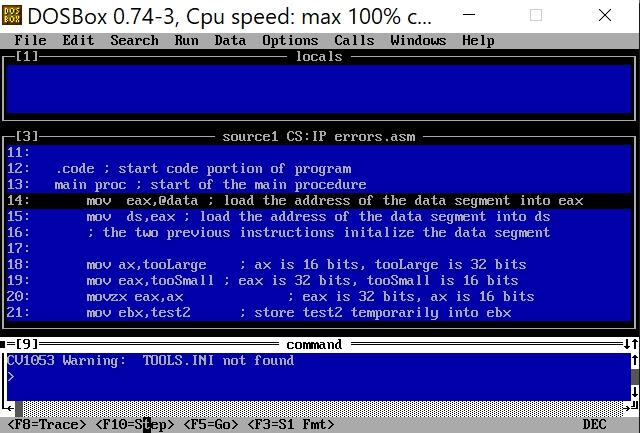
\includegraphics[width=\linewidth]{images/firstCV.jpg}
  \caption{Initial CodeView Screen.}
  \label{fig:cv1}
\end{figure}
A screen like this one (Figure \ref{fig:cv1}) will pop up. 
The next thing we will do is open the Register window (click {\code Windows -> Register}).  Since we have one memory location changing we'll add a Watch (click {\code Data->Add Watch} and type in test1 and hit ok).  
\begin{figure}
  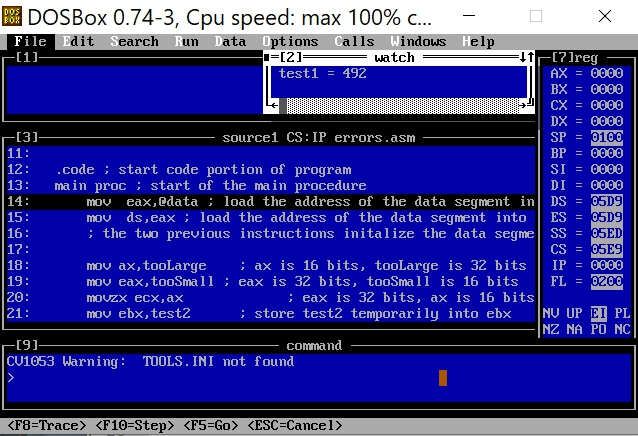
\includegraphics[width=\linewidth]{images/watchCV.jpg}
  \caption{CodeView with Registers and a Watch.}
  \label{fig:cv2}
\end{figure}
The window now should look like this (Figure \ref{fig:cv2}). 

Now we can step through our code and see how the registers change, hit F10 to step through each line.  When the program is through, it has the final values of the registers, a garbage value for test1 since the program is over, and gives a peek at the assembled code (Figure \ref{fig:cv3}).  
\begin{figure}
  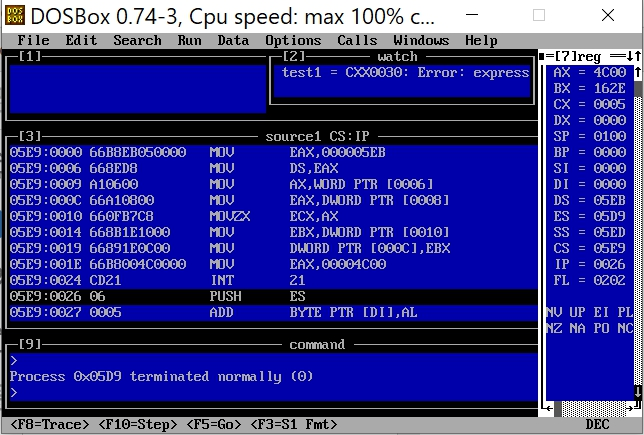
\includegraphics[width=\linewidth]{images/endCV.jpg}
  \caption{CodeView after program runs.}
  \label{fig:cv3}
\end{figure}
Just like in most IDEs you are used to you can also set break points instead of running every line and once you have procedures you can use F8 to trace the procedure or F10 to step over it.  
% do fib for lecture and debug it on the fly do errors for this to show registers and memory
%
\subsection{DOSBox/MASM Quirks}
\begin{itemize}
\item Sometimes your mouse will get stuck in the DOSBox window if you hit alt-Tab that will switch to another open window on your computer and will free your mouse. 
\item If you have an infinite loop or otherwise want to force your program to close, the best way is to just close DOSBox altogether and restart. 
\item In CodeView sometimes it will stop recognizing the mouse, but the keyboard will still work so you can use the shortcut keys.  If you need to choose something from the Menu you can type Alt-F to open the File Menu then you can use the arrow keys and then enter to select what you need.  To exit you can simply type Alt-F4.    
%more?
\end{itemize}